\clearpage
% \setcounter{page}{1}
\maketitlesupplementary
\begin{figure*}[htbp]
    \centering
    \includegraphics[width=1.0\linewidth]{solver_hw_v5.pdf}
    \caption{Illustration of Part Solver Module.}
    \label{fig:solver}
\end{figure*}
\section{Method Details}
This section provides additional implementation and methodological details of FreeArtGS:
\begin{itemize}
    \item Sec.~\ref{sec:init}: the initialization procedure of the rigid transformations in part segmentation.
    \item Sec.~\ref{sec:filter}: the trajectory filtering strategy to obtain a reliable subset of trajectories given the point-tracking priors.
    \item Sec.~\ref{sec:partseg}: the propagation algorithm from optimized part weights to segmentations.
    \item Sec.~\ref{sec:camera}: additional description of part pose estimation.
    \item Sec.~\ref{sec:jointtype}: the criterion of deciding the joint type.
    \item Sec.~\ref{sec:jointaxis}: the strategy of estimating the joint axis.
\end{itemize}
Figure~\ref{fig:solver} further illustrates the detailed data flow of the Part Solver module introduced in Sec.~3.2 of the main paper.

% We provide a more detailed illustration of the Part Solver in Figure~\ref{fig:solver}, which elaborates on the high-level pipeline shown in Figure~\ref{fig:pipeline}. In particular, we describe the \textbf{} and \textbf{Filter and Fill in Trajectories} components.

\subsection{Transformation Initialization}
\label{sec:init}
As described in Sec. 3.2 of the manuscript, our method processes the input video in a window-wise manner. 
Before each optimization procedure, the rigid transformations must be initialized for the corresponding frame pairs within the window.

For each frame pair $(t, t{+}x)$ with $x \in [1, K-1]$, where $K$ is the window size, let $X_{t,p}$ and $X_{t+x,p}$, with $p\in\mathcal{P}$, denote the 3D positions of trajectory point $p$ at times $t$ and $t{+}x$, respectively. 
Given an initial partition of the trajectories into two parts, $\mathcal{P}_0$ and $\mathcal{P}_1$, we estimate the rigid transforms $T^0_{t\to t+x}, T^1_{t\to t+x} \in \mathrm{SE}(3)$ by minimizing a robust registration objective:
\begin{equation}
    T^k_{t\to t+x}
    = \arg\min_{T \in \mathrm{SE}(3)} 
    \sum_{p \in \mathcal{P}_k} 
    \rho\big(\,\lVert X_{t+x,p} - T X_{t,p} \rVert_2^2\big),
    \label{eq:init_reg}
\end{equation}
where $\rho(\cdot)$ denotes the Tukey loss. 
In practice, we realize this step with a RANSAC-based estimator followed by refinement under the Tukey weighting scheme, which increases robustness to outliers.

To further improve the initialization, we perform an EM-style iterative refinement over trajectory assignments and transforms. 
Let $z_p \in \{0,1\}$ denote the part label of trajectory $p$. 
At iteration $i$, the E-step assigns each trajectory to the transform with the smaller reconstruction error:
\begin{equation*}
    z_p^{(i+1)} 
    = \arg\min_{k \in \{0,1\}} 
    \lVert X_{t+x,p} - T^{k,(i)}_{t\to t+x} X_{t,p} \rVert_2^2
    \label{eq:em_estep}
\end{equation*}
In the M-step, the transforms are re-estimated given the updated assignments by solving
\begin{equation*}
    T^{k,(i+1)}_{t\to t+x} 
    = \arg\min_{T} 
    \sum_{p : z_p^{(i+1)} = k} 
    \rho\big(\,\lVert X_{t+x,p} - T X_{t,p} \rVert_2^2\big)
    \label{eq:em_mstep}
\end{equation*}
The final estimates are used as the initial transformations $T^0_{t\to t+x}$ and $T^1_{t\to t+x}$ for frame pair $(t,t{+}x)$, providing a robust starting point that reduces the risk of convergence to poor local optima.

\subsection{Trajectory Filtering}
\label{sec:filter}
The off-the-shelf point tracking model~\cite{alltracker} can produce noisy trajectories, and directly using all trajectories $\{X_{t,p}\}$ is suboptimal. We therefore apply a multi-stage filtering scheme to obtain a reliable subset of trajectories.

We first retain trajectories that remain visible and inside the foreground masks across frames. 
Let $c_{t,p}$ denote the visibility confidence of trajectory $p$ at time $t$ predicted by the point tracking model, and let $m_{t,p} \in \{0,1\}$ indicate whether the corresponding pixel lies inside the foreground mask at time $t$. 
We define the visibility- and mask-consistent set as
\begin{equation}
    \mathcal{S}_{\mathrm{vis}}
    = \big\{ (t,p) \,\big|\,
        c_{t,p} > \tau_c,\;
        m_{t,p} = 1,\;
        m_{t+1,p} = 1
      \big\},
\end{equation}
where $\tau_c=0.5$ is a visibility threshold.

To further suppress motion outliers, we filter trajectories by displacement magnitude. 
Let $\Delta X_{t,p} = X_{t+1,p} - X_{t,p}$ and denote the mean and standard deviation of $\lVert \Delta X_{t,p} \rVert_2$ over $(t,p) \in \mathcal{S}_{\mathrm{vis}}$ as $\mu_v$ and $\sigma_v$, respectively. 
We keep
\begin{equation*}
    \mathcal{S}_{\mathrm{final}}
    = \big\{ (t,p) \in \mathcal{S}_{\mathrm{vis}} \,\big|\,
        \lVert \Delta X_{t,p} \rVert_2 
        \le \mu_v + \tau_v \sigma_v
      \big\},
\end{equation*}
where $\tau_v=2$ is a displacement threshold. 

\subsection{Part Segmentation}
\label{sec:partseg}
% followed by a feature-based filling step to propagate part information to the full foreground.
% The propagation procedure from part weights to segmentations
% After the optimization iterations of the part solver, each selected trajectory $(t,p) \in \mathcal{S}_{\mathrm{final}}$ is associated with a part weight $w_{t,p} \in [0,1]$. 
To propagate the part weights from sparse trajectories to the full-pixel map, we leverage DINO features for semantic-aware interpolation. 
Let $\phi_t(u)$ denote the DINO feature at pixel $u$ in frame $t$, and let $\mathcal{U}_t$ be the set of foreground pixels that are not directly covered by the retained trajectories. 
For each $u \in \mathcal{U}_t$, we first compute the cosine similarity between $u$ and each trajectory point:
\begin{equation*}
    s_t(u,p)
    = \cos\!\big(\phi_t(u), \phi_t(p)\big)
    = \frac{\phi_t(u)^\top \phi_t(p)}
           {\lVert \phi_t(u) \rVert_2 \,\lVert \phi_t(p) \rVert_2},
\end{equation*}
The interpolated part weight at pixel $u$ is then defined as the similarity-weighted average
\begin{equation*}
    \tilde{w}_t(u)
    = \frac{
        \sum_p
        s_t(u,p)\, w_{t,p}
    }{
        \sum_p
        s_t(u,p)
    }.
\end{equation*}
The resulting dense part weight map $\tilde{w}_t$ is passed to the next window.

\subsection{Part Pose Estimation}
\label{sec:camera}
As previously discussed, we adopt an off-the-shelf approach to estimate part-to-camera poses, exemplified by BundleSDF~\cite{bundlesdf}. For improved accuracy on synthetic datasets, we replace the feature-matching stage in the Coarse Pose Initialization module of the BundleSDF pipeline with an ICP-based procedure. This adjustment is motivated by the fact that objects in simulation typically exhibit extremely limited texture—many are nearly monochromatic—rendering feature matching unreliable.
For real-world objects, however, we retain the original BundleSDF pipeline unchanged, as it demonstrates robust performance under such conditions.
\subsection{Joint Type Estimation}
\label{sec:jointtype}
We propose a simple criterion to decide whether a motion sequence
should be modeled as a revolute joint or a prismatic joint, based only on
the observed part poses. The decision is made using two scalar features: \textbf{Rotation Amplitude} and \textbf{Translation Linearity Ratio}. We describe the decision criterion as follows.

\paragraph{Input.}
We are given a sequence of relative part poses
\[
T_i \in SE(3), \quad i = 1,\dots,N,
\]
where
\(
T_i =
\begin{bmatrix}
R_i & t_i \\
0 & 1
\end{bmatrix},
\; R_i \in SO(3),\; t_i \in \mathbb{R}^3.
\)
Each $R_i$ is projected to $SO(3)$ to remove numerical noise.

\paragraph{Rotation Amplitude.}
We first measure how much the object rotates over the whole sequence.

We compute the mean rotation by projecting the sum of rotations to
$SO(3)$:
\[
S = \sum_{i=1}^N R_i, \quad
S = U \Sigma V^\top, \quad
R_{\mathrm{mean}} = U V^\top \in SO(3).
\]
For each frame, we form the relative rotation to the mean,
\[
R_i^{\mathrm{rel}} = \operatorname{Proj}_{SO(3)}\!\bigl(R_i R_{\mathrm{mean}}^\top\bigr),
\]
and convert it to an angle
\[
\theta_i = \arccos\!\Bigl(\tfrac{1}{2}(\operatorname{tr}(R_i^{\mathrm{rel}})-1)\Bigr).
\]

To obtain a robust rotation span, we apply an IQR-based outlier
rejection to the set $\{\theta_i\}$ and then define
\[
\Delta\theta = 
\max_{\theta \,\text{inliers}} \theta \;-\;
\min_{\theta \,\text{inliers}} \theta,
\]
and convert it to degrees
\[
\Delta\theta_{\mathrm{deg}} = \frac{180}{\pi}\,\Delta\theta.
\]
This scalar $\Delta\theta_{\mathrm{deg}}$ measures the overall
\textit{rotation amplitude} of the sequence.

\paragraph{Translation Linearity Ratio.}
Independently, we analyze how linear the translation trajectory is.
We first center the translations,
\[
\bar{t} = \frac{1}{N}\sum_{i=1}^N t_i, \quad
x_i = t_i - \bar{t},
\]
and build the (unnormalized) covariance matrix
\[
C = \sum_{i=1}^N x_i x_i^\top \in \mathbb{R}^{3\times 3}.
\]
Let its eigenvalues in descending order be
\[
\lambda_1 \ge \lambda_2 \ge \lambda_3 \ge 0.
\]
We define a \emph{translation linearity ratio}
\[
\rho = \frac{\lambda_2 + \lambda_3}{\lambda_1 + \varepsilon},
\]
with a small $\varepsilon > 0$ to avoid division by zero.
When the translations lie close to a single straight line, $\lambda_1$
dominates and $\rho$ becomes small.

\paragraph{Decision Criterion.}
Using these two scalar features, we classify the joint type according to
\[
\text{model} =
\begin{cases}
\text{prismatic}, 
& \text{if } \Delta\theta_{\mathrm{deg}} < \theta_{\mathrm{th}}
\;\; \text{or} \;\; \rho < \rho_{\mathrm{th}},\\[4pt]
\text{revolute},
& \text{otherwise}.
\end{cases}
\]
In our implementation, we set
\(
\theta_{\mathrm{th}} = 10^\circ
\)
and
\(
\rho_{\mathrm{th}} = 0.05.
\)

Intuitively, if the object barely rotates (small
$\Delta\theta_{\mathrm{deg}}$), or if its translation is very close
to a straight line in 3D (small $\rho$), the motion is better
explained by a prismatic joint; otherwise we adopt a revolute-joint
model.

\begin{table*}[t]

\centering
\caption{Results of Robustness Analysis.}
\label{tab:more_ablation}
\renewcommand\tabcolsep{7pt}
% \setlength{\tabcolsep}{3pt}
% \scriptsize
\resizebox{\linewidth}{!}{%
\begin{tabular}{llcccccccc}
\toprule
\textbf{Joint Type} & \textbf{Method} & \boldmath\textbf{Axis(deg)$\downarrow$} & \boldmath\textbf{Position(cm)$\downarrow$} & \boldmath\textbf{State(deg/cm)$\downarrow$} & \boldmath\textbf{CD-w(cm)$\downarrow$} & \boldmath\textbf{CD-m(cm)$\downarrow$} & \boldmath\textbf{CD-s(cm)$\downarrow$} & \boldmath\textbf{PSNR(dB)$\uparrow$} \\
\midrule
\multirow{4}{*}{\centering Revolute} 
& 2\% Depth Noise & 1.41$\pm$1.49 & 0.51$\pm$0.58 & 1.22$\pm$1.27 & 0.23$\pm$0.30 & 0.30$\pm$0.27 & 1.05$\pm$2.47 & 23.52$\pm$4.65 \\
% & 5\% Depth Noise & 9.35$\pm$13.50 & 19.58$\pm$39.17 & 14.64$\pm$19.90 & 0.75$\pm$0.90 & 1.90$\pm$3.11 & 1.14$\pm$2.60 & 13.07$\pm$7.26 \\
& AllTracker $\to$ CoTracker3& \textbf{0.88$\pm$0.84} & 0.46$\pm$0.86 & 1.68$\pm$1.30 & 0.79$\pm$2.19 & 0.80$\pm$1.08 & 1.47$\pm$2.43 & 23.87$\pm$4.94 \\
& DINOv3 $\to$ DINOv2 & 1.64$\pm$1.22 & 0.32$\pm$0.47 & \textbf{1.21$\pm$0.77} & \textbf{0.11$\pm$0.11} & \textbf{0.28$\pm$0.27} & 1.04$\pm$2.52 & 23.74$\pm$4.41 \\
& \textbf{Ours} & 1.04$\pm$1.03 & 
\textbf{0.29$\pm$0.36} & 1.43$\pm$1.20 & 0.14$\pm$0.13 & 0.28$\pm$0.36 & \textbf{0.97$\pm$2.69} & \textbf{24.02$\pm$3.15} \\
\midrule
\multirow{4}{*}{\centering Prismatic} 
& 2\% Depth Noise & 1.86$\pm$2.51 & - & 0.92$\pm$0.66 & \textbf{0.34$\pm$0.13} & 1.07$\pm$1.18 & 1.78$\pm$3.03 & 21.75$\pm$2.99 \\
% & 5\% Depth Noise & 28.72$\pm$27.83 & - & 38.31$\pm$38.81 & 22.3$\pm$50.18 & 23.73$\pm$44.37 & 21.62$\pm$45.33 & 13.86$\pm$4.48 \\
& AllTracker $\to$ CoTracker3 & 1.98$\pm$3.09 & - & 1.12$\pm$0.68 & 0.79$\pm$1.08 & 0.98$\pm$1.22 & 0.94$\pm$1.18 & 21.85$\pm$3.64 \\ %TODO
& DINOv3 $\to$ DINOv2 & \textbf{1.46$\pm$1.63} & - & 0.96$\pm$1.59 & 0.56$\pm$0.40 & 0.99$\pm$0.93 & 0.46$\pm$0.51 & 22.39$\pm$3.92 \\
& \textbf{Ours} & 1.85$\pm$2.75 & \textbf{-} & \textbf{0.90$\pm$0.53} & 0.41$\pm$0.22 & \textbf{0.67$\pm$0.34} & \textbf{0.30$\pm$0.13} & \textbf{22.92$\pm$2.65} \\
\bottomrule
\end{tabular}%
}
\end{table*}

\subsection{Joint Axis Estimation}
\label{sec:jointaxis}
Given a sequence of relative part poses 
\[
    T_i = 
    \begin{bmatrix}
        R_i & t_i\\
        0 & 1
    \end{bmatrix}
    \in SE(3), \quad i=1,\dots,N,
\]
our goal is to estimate the underlying joint axis.
Depending on the joint type inferred in the previous stage, we adopt two different strategies, described below.

\paragraph{Revolute Model.}
For a fixed-axis (revolute) joint, all rotations share a common axis direction.
Let 
\[
    R_{ij} = \operatorname{Proj}_{SO(3)}(R_i R_j^\top)
\]
denote the relative rotation between frames $i$ and $j$, where $\operatorname{Proj}_{SO(3)}$ removes numerical drift.
In an ideal revolute motion, the unknown axis direction $u$ satisfies
\[
    R_{ij} u = u
    \quad\Longleftrightarrow\quad
    (R_{ij}-I)\,u = 0
    \quad\forall\, i<j.
\]
Thus $u$ lies in the approximate null space shared by all matrices $(R_{ij}-I)$.
We therefore minimize the quadratic error
\[
    u^\star = 
    \arg\min_{\|u\|=1}
    \sum_{i<j}
        \|(R_{ij} - I)u\|^2.
\]
Expanding the objective yields the symmetric matrix
\[
    A = 
    \sum_{i<j}
        (R_{ij}-I)^\top (R_{ij}-I),
\]
whose eigenvector associated with the smallest eigenvalue gives the optimal axis direction,
\[
    A u^\star = \lambda_{\min} u^\star,
    \qquad \|u^\star\| = 1.
\]

Once the axis direction is known, the axis point $p$ is estimated from the translational consistency equation for a rigid rotation without screw pitch:
\[
    t_i \approx c + (I - R_i)p.
\]
Subtracting two frames removes the global offset $c$:
\[
    t_i - t_j \approx (R_j - R_i)p.
\]
Since the component of $p$ along $u$ is unobservable, we solve $p$ in the plane orthogonal to $u$.  
Let $P = I - u u^\top$ be the projection onto $u^\perp$, then
\[
    P(t_i - t_j) \approx P(R_j - R_i)p.
\]
Stacking all such constraints yields a least-squares system, whose solution is projected back onto $u^\perp$ to enforce $u^\top p = 0$, giving a unique axis point closest to the origin.

\paragraph{Prismatic Model.}
For a prismatic joint, the rigid body exhibits negligible rotation while its translations $\{t_i\}$ lie approximately on a straight 3D line.
We estimate the sliding direction and axis point from the translational trajectory.

Translations are first centered:
\[
    \bar t = \frac{1}{N}\sum_{i=1}^N t_i,
    \qquad
    x_i = t_i - \bar t.
\]
The covariance matrix
\[
    C = \sum_{i=1}^N x_i x_i^\top
\]
is decomposed as
\[
    C v_k = \lambda_k v_k,
    \qquad
    \lambda_1 \ge \lambda_2 \ge \lambda_3 \ge 0.
\]
If the motion is prismatic, $\lambda_1$ dominates, and the first principal component encodes the translation line direction.  
Thus the prismatic axis is
\[
    w^\star = \frac{v_1}{\|v_1\|}.
\]

The axis point $p_0$ is the closest point on this line to the origin, obtained by projecting the mean translation onto $w^\star$:
\[
    p_0 
    = \bar t - (\bar t^\top w^\star)\, w^\star.
\]
Each frame’s joint displacement is then the signed projection
\[
    d_i = (t_i - p_0)^\top w^\star,
\]
which, together with a constant rotation offset, fully characterizes the prismatic motion.



\section{Benchmark Details of FreeArt-21}

We provide further details about the FreeArt-21 benchmark in this section. All data are collected through tele-operation within the Sapien simulator~\cite{partnetmobility}. A human operator simultaneously controls the 6-DoF poses and joint parameters of articulated objects using a PICO 4 Ultra VR headset and controllers, enabling real-time manipulation and interaction with the objects. The camera is positioned approximately 3 meters away from the object in simulation, providing a realistic perspective for the data collection. Each case in the benchmark contains multi-modal data, including RGB images, depth maps, ground-truth object and part masks, as well as the 6-DoF object poses and joint parameters. These elements provide rich supervision for training and evaluating object pose estimation and articulated manipulation tasks. The data collection involves between 200 and 400 frames per sequence, capturing diverse interaction patterns. 

Compared to other datasets, FreeArt-21 offers more human-like data collection, as the sequences are captured through human teleoperation, rather than automated generation or pre-set trajectories, making it more representative of real-world scenarios where objects are scanned by a person. The objects included in FreeArt-21 are shown in Figure~\ref{fig:benchmark}.

\section{Additional Experiment Results}

\subsection{Robustness Analysis}
We further evaluate the robustness of our framework by replacing AllTracker with CoTracker3 and DINOv3 with DINOv2, while also injecting 2\% Gaussian noise into the depth of the FreeArt-21 dataset. As shown in Table~\ref{tab:more_ablation}, the results indicate that FreeArtGS remains robust to noisy depth inputs and variations in predictions from upstream models.

\subsection{Camera Pose Estimation Results}
We evaluate our camera pose estimation results on the Video2Articulation-S dataset and compare them with the baseline method, Video2Articulation~\cite{video2articulation}. Camera pose is a crucial variable that is jointly optimized in our end-to-end pipeline. As shown in Table~\ref{tab:results_video2articulation_cam}, our method achieves significantly lower rotation and translation errors than the baseline, resulting in a more accurate reconstruction of the articulated objects.
We also provide trajectory visualizations in Figure~\ref{fig:camera pose vis} to qualitatively show the alignment between estimated and ground-truth trajectories.

\begin{table}[h]
    \centering
    \caption{Results of Camera Pose Estimation on the Video2Articulation-S Dataset. * indicates that the results are taken from the original paper.}
    \label{tab:results_video2articulation_cam}
    \renewcommand\tabcolsep{7pt}
    \resizebox{\linewidth}{!}{%%
    \begin{tabular}{lcc}
    \toprule
    \textbf{Method} & \boldmath\textbf{Rot. Error (deg)$\downarrow$} & \boldmath\textbf{Pos. Error (cm)$\downarrow$} \\
    \midrule
    {Video2Articulation*~\cite{video2articulation}} & 4.621 & 9.246 \\
    \textbf{Ours} & \textbf{2.483} & \textbf{1.526} \\
    \bottomrule
    \end{tabular}%
}
\end{table}

\begin{figure}[htbp]
    \centering
    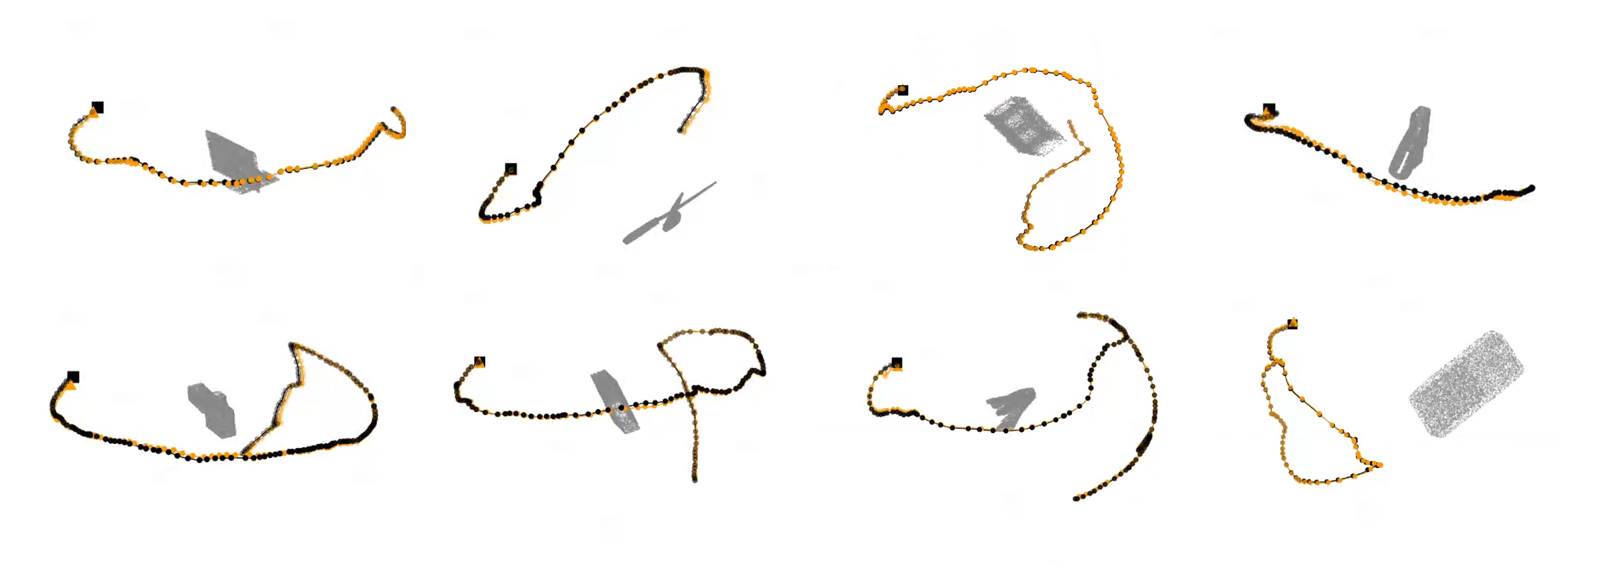
\includegraphics[width=1\linewidth]{campose_vis.png}
    \caption{Visualization of camera pose trajectories in FreeArt-21. The black line shows the ground truth camera trajectory, and the yellow line shows our estimated camera trajectory. }
    \label{fig:camera pose vis}
\end{figure}

\subsection{Part Segmentation Results}
We additionally report the evaluation of our part segmentation. The metrics are calculated in terms of mIoU of the two parts in Table~\ref{tab:iou}. This result confirms that our model produces consistent part segmentations that align closely with the annotated masks.

\begin{table}[h]
    \centering
    \caption{Results of Part Segmentation. * indicates that the results are taken from the original paper.}
    \label{tab:iou}
    \renewcommand\tabcolsep{7pt}
    \resizebox{\linewidth}{!}{%%
    \begin{tabular}{lcc}
    \toprule
    \textbf{Method / mIoU (\%)$\uparrow$} & \textbf{FreeArt-21} & \textbf{Video2Articulation-S} \\
    \midrule
    {Video2Articulation~\cite{video2articulation}} & 34.61 & 59.65* \\
    \textbf{Ours} & \textbf{90.88} & \textbf{84.92} \\
    \bottomrule
    \end{tabular}%
}
\end{table}

\subsection{More Visualization on FreeArt-21}
% We provide additional visualizations for all other cases in FreeArt-21 in Figure~\ref{fig:all_vis}.
We visualize more reconstruction results on FreeArt-21 in Figure~\ref{fig:all_vis}. 

%  \subsection{Quantitative Results on Real Objects}
% We annotate the articulation axes of the real-world objects and report the corresponding metrics in Tab.~\ref{tab:quantitative results of real}. Chamfer Distance (CD) is computed from the ground-truth and rendered depth point clouds for each frame. The ground-truth axes and positions are obtained through manual annotation. Following our annotation protocol, the rotation and translation errors are clipped to $0.1^\circ$ and $0.1$ cm, respectively, which correspond to the smallest annotation units.

% \begin{table}[t]
%     \centering
%     \caption{Results of reconstruction on real-world objects. }
   
%     \label{tab:quantitative results of real}
%     \renewcommand\tabcolsep{7pt}
%     \resizebox{0.48\textwidth}{!}{%%
%     \begin{tabular}{lcccc}
%     \toprule
%     Objects & Axis (deg)$\downarrow$ & Position (cm)$\downarrow$ & CD (cm)$\downarrow$ & PSNR (dB) $\uparrow$ \\
%     \midrule
%     Box & 0.10 & 0.10 & 1.89 &  22.77  \\
%     Drawer & 1.06 & - & 1.91 &  19.82  \\
%     Bin & 4.68 & 0.20 & 3.46 & 23.75   \\
%     Fan & 1.53 & 1.30 & 1.78 &  21.95  \\
%     Door & 0.10 & 3.30 & 2.53 &  23.71  \\
%     Lid & 8.92 & 0.40 & 3.36 & 22.39   \\
%     \textbf{Average} & 2.73 & 1.06 & 2.48 & 22.40\\
%     \bottomrule
%     \end{tabular}%
%     }
% \end{table}

% \begin{figure*}[t]
%     \centering
%     \includegraphics[width=1.0\linewidth]{iou.pdf}
%     \caption{Visualization of Part Segmentation in FreeArt-21. The first row shows the ground truth RGB image. The following 2 rows are masks of 2 parts. The last row presents the map of part weights $w$.}
%     \label{fig:iou}
% \end{figure*}
\section{Failure Case Analysis}

\noindent\textbf{Part Segmentation Failures.} Our pipeline's efficacy is closely tied to the accuracy of part segmentation. In cases involving narrow or elongated structures or objects with extremely low texture, the tracked 3D trajectories often exhibit significant drift. These deviations potentially bias the motion-based clustering toward incorrect part assignments. Such mis-segmentation directly undermines the subsequent joint estimation and geometry reconstruction.

\noindent\textbf{Part Pose Ambiguities.} The precision of articulation axis estimation and surface reconstruction is also highly sensitive to part pose accuracy. While we initialize poses using off-the-shelf methods and refine them during optimization, thin or planar objects (e.g., monitors or scissors) present significant challenges. The scarcity of reliable feature correspondences on these geometries often leads to poorly constrained pose optimization. Consequently, the resulting articulation axes may deviate from the physical ground truth, and the reconstructed geometry may suffer from noticeable structural artifacts.

% Our pipeline relies heavily on the ability of part segmentation to isolate the components of articulated objects accurately. When the object contains narrow or elongated surfaces/parts or exhibits extremely low texture, the 3D trajectories produced by tracking often deviate significantly. Such deviations cause a subset of points to be optimized toward incorrect part labels during the segmentation stage.

% Another critical factor influencing axis estimation and reconstruction quality is the camera pose. We employ the off-the-shelf methods to compute camera poses independently for different parts and optimize them in the following reconstruction. However, for thin or planar objects (e.g., monitors, scissors), the limited number of reliable correspondences often makes it difficult to obtain accurate camera poses. Consequently, the estimated articulation axes and the reconstructed geometry can suffer from noticeable errors.

\begin{figure*}[t]
    \centering
    \includegraphics[width=1\linewidth]{benchmark.pdf}
    \caption{Visualization of all objects in FreeArt-21. }
    \label{fig:benchmark}
\end{figure*}

\begin{figure*}[b]
    \centering
    \includegraphics[width=1.0\linewidth]{vis_all_hw.pdf}
    \caption{Visualization of our reconstruction results on FreeArt-21.}
    \label{fig:all_vis}
\end{figure*}
% \section{Additional Results on Real Objects}

% \section{Additional Implementation Details}
% \label{sec:Inplementation}
% \subsection{Baselines}

